% =====================================================================
%  Fair Outside, Loaded Inside -- first draft
%  Compile:  latexmk -pdf main.tex      (VS Code + LaTeX Workshop: just save)
%
%  FIGURES: put this file in your project folder and point \figdir at the
%  folder that holds your plots (relative to this file). Then edit the file
%  names in the "FIGURE FILES" block below. Any figure that is not found is
%  drawn as a labelled grey box, so the PDF always compiles.
%
%  REFERENCES: keep refs.bib in the same folder as this file.
% =====================================================================
\documentclass[conference]{IEEEtran}
\IEEEoverridecommandlockouts

\usepackage{amsmath,amssymb,amsfonts}
\usepackage{graphicx}
\usepackage{textcomp}
\usepackage{xcolor}
\usepackage{booktabs}
\usepackage{tikz}
\usetikzlibrary{positioning,arrows.meta}
\usepackage{url}
\usepackage{cite}
\usepackage{placeins} % \FloatBarrier

% ---------------------------------------------------------------------
%  FIGURE FILES  (edit these to match your project directory)
% ---------------------------------------------------------------------
\newcommand{\figdir}{figures/}   % e.g. results/figures/  (keep the trailing /)
\newcommand{\repourl}{\url{https://github.com/bijyeta-maharjan/disentangling-speaker-sex-encoding-and-use}}

\newcommand{\FigSexAccent}{sex_accent_heatmap.png}      % slide 3 left
\newcommand{\FigFzero}{f0_by_sex.png}                    % slide 3 right
\newcommand{\FigLeakage}{leakage_gap.png}                % slide 6 left
\newcommand{\FigAccBySex}{accuracy_by_sex.png}           % slide 7
\newcommand{\FigProbeSex}{probe_layerwise_sex.png}       % slide 11
\newcommand{\FigProbeId}{probe_layerwise_speaker.png}    % slide 12
\newcommand{\FigSeedMargins}{seed_margins.png}           % slide 23
\newcommand{\FigNecessity}{necessity_all_arch.png}       % slide 26
\newcommand{\FigDftLrp}{dftlrp_band_share.png}           % slide 28
\newcommand{\FigFaithful}{dftlrp_faithfulness.png}       % slide 29
\newcommand{\FigSplitNull}{whitened_direction_null.png}  % slide 43
\newcommand{\FigFzeroProj}{direction_vs_f0.png}          % slide 45
\newcommand{\FigJacobian}{readout_jacobian_heatmap.png}  % slide 46
\newcommand{\FigCounterfactual}{counterfactual_shift.png}% slide 47
\newcommand{\FigMaleOnly}{male_only_gap.png}             % slide 50
\newcommand{\FigFtRecovery}{finetune_recovery.png}       % slide 54
\newcommand{\FigFtBands}{finetune_band_change.png}       % slide 56

% \paperfig[width]{file}: include if it exists, otherwise draw a placeholder
\newcommand{\paperfig}[2][\linewidth]{%
  \edef\pfname{#2}%
  \IfFileExists{\figdir\pfname}%
    {\includegraphics[width=#1,keepaspectratio]{\figdir\pfname}}%
    {\fbox{\parbox[c][0.45#1][c]{\dimexpr#1-2\fboxsep-2\fboxrule}{\centering
      \footnotesize\color{gray}Missing figure\\
      \texttt{\expandafter\detokenize\expandafter{\pfname}}}}}}

% \paperfigh[height]{file}: same, but sized by height (for panel grids)
\newcommand{\paperfigh}[2][4cm]{%
  \edef\pfname{#2}%
  \IfFileExists{\figdir\pfname}%
    {\includegraphics[height=#1,keepaspectratio]{\figdir\pfname}}%
    {\fbox{\parbox[c][#1][c]{4cm}{\centering\footnotesize\color{gray}Missing
      figure\\\texttt{\expandafter\detokenize\expandafter{\pfname}}}}}}

% Draft notes (set \drafttrue to \draftfalse to hide them)
\newif\ifdraft \draftfalse
\newcommand{\todo}[1]{\ifdraft{\color{red}\textbf{[TODO:} #1\textbf{]}}\fi}

% Let LaTeX place more figures per page so they stay near their text
\renewcommand{\topfraction}{0.9}
\renewcommand{\dbltopfraction}{0.9}
\renewcommand{\bottomfraction}{0.8}
\renewcommand{\textfraction}{0.07}
\renewcommand{\floatpagefraction}{0.75}
\renewcommand{\dblfloatpagefraction}{0.75}
\setcounter{topnumber}{3}
\setcounter{dbltopnumber}{3}
\setcounter{totalnumber}{5}

\begin{document}

\title{Disentangling Speaker Sex Encoding and Use\\ in Spoken-Digit Classifiers}

\author{
\IEEEauthorblockN{Bijyeta Maharjan}
\IEEEauthorblockA{\textit{Computer Science} \\ \textit{Mount Holyoke College} \\
South Hadley, MA, USA \\ mahar25b@mtholyoke.edu}
\and
\IEEEauthorblockN{Supervisor: Dr.\ Nils Gumpfer}
\IEEEauthorblockA{\textit{AAI Lab} \\ \textit{Technische Hochschule Mittelhessen} \\
Friedberg, Germany \\ nils.gumpfer@kite.thm.de}
}

\maketitle

% =====================================================================
\begin{abstract}
Fairness audits of speech models usually check whether accuracy is equal
across demographic groups. Equal accuracy, however, says nothing about
whether a model internally encodes a protected attribute, or whether its
decisions depend on it. We separate these two claims, \emph{encoded} and
\emph{used}, in a controlled study of spoken-digit classification on
AudioMNIST, across four architectures and three training seeds. Linear
probes recover speaker sex from the convolutional networks with up to 99\%
accuracy, yet an untrained copy of each network decodes sex just as well: the
information is inherited from the audio, not induced by training. Frequency occlusion and
faithfulness-checked DFT-LRP show that digit decisions rely on the formant
region below 750\,Hz. Sex-probe directions lie 79--90$^\circ$ from the
digit decision at every layer. For a sex direction validated against an
exhaustive null of 219 speaker re-splits, the readout's sensitivity never
exceeds the 95th percentile of random directions (0 of 60 tests), and
shifting representations along it leaves accuracy unchanged.
Behaviourally, a model trained only on male speakers still loses 5--8 points
on unseen female speakers, and fine-tuning recovers this through late-layer
recalibration rather than frequency-selective change. All sex-related claims
rest on three held-out female speakers, which we treat as a hard ceiling.
\end{abstract}

\begin{IEEEkeywords}
explainable AI, algorithmic fairness, probing, concept directions, speech
classification, AudioMNIST
\end{IEEEkeywords}

% =====================================================================
\section{Introduction}

Machine-learning models that listen to people, from voice assistants to
clinical monitoring of speech and physiological signals, are increasingly
used in settings where unequal performance has real costs. Documented
accuracy gaps by sex and dialect in automatic speech recognition
\cite{tatman2017gender,koenecke2020racial} have made group-level accuracy the
default fairness check for such systems \cite{hardt2016equality}.

The difficulty is that output parity cannot tell a model that ignores a
protected attribute apart from one that uses it in ways that happen to
balance out. A voice carries its speaker's sex and identity whether or not
the task needs them, and networks readily exploit any pattern that helps
\cite{geirhos2020shortcut}. Even with balanced data, internal
representations can still carry demographic information
\cite{wang2019balanced}.

Current tools each see part of the picture. Group metrics see only outputs.
Probing classifiers show that information is \emph{present} in a
representation, but not that the model relies on it
\cite{belinkov2022probing,hewitt2019control}. Input attribution methods
\cite{bach2015lrp,vielhaben2024virtual} score which input features drive a
decision, but struggle when the task cue and the demographic cue occupy the
same frequencies, as pitch and formants do in speech.

We therefore run a mechanistic study that tests \emph{encoded} and
\emph{used} as separate, falsifiable claims, at three levels: the input
spectrum, the internal representation and the model's behaviour. We use
AudioMNIST \cite{becker2024audiomnist} as a transparent sandbox, before
moving the method to clinical time series.

Our contributions are: (i) an encoded-vs-used protocol with untrained-network
and raw-input controls, replicated over four architectures and three seeds;
(ii) convergent input-level evidence from band occlusion and
faithfulness-checked DFT-LRP; (iii) direction-level evidence of non-use, based
on a sex direction validated against an exhaustive split null and
tested by geometry, readout sensitivity and counterfactual shifts; and (iv) a
reconciliation of these results with a sex-linked behavioural gap, localised
to late-layer recalibration. Section~\ref{sec:problem} states the problem,
Sections~\ref{sec:objective}--\ref{sec:related} give the objective, research
questions and related work, Section~\ref{sec:method} the methodology,
Section~\ref{sec:results} the results, Section~\ref{sec:conclusion} the
conclusions and Section~\ref{sec:future} future work.

% =====================================================================
\section{Problem Statement}\label{sec:problem}

\emph{Group-accuracy parity does not reveal whether a speech classifier
encodes speaker sex, nor whether its decisions depend on it. The gap
addressed here is how to test encoding and use as separate claims, each with
its own control, in a setting small enough to be inspected fully.}

The scope is spoken-digit classification on AudioMNIST, speaker sex and
speaker identity as attributes, four architectures, and linear read-outs of
internal representations. Accent and age are out of scope, because the
dataset does not contain enough speakers per group. A population-level
fairness verdict is also out of scope, for the reason below.

The problem is hard for three reasons. First, the digit and sex cues overlap
in the same low-frequency band, so removing one input region removes both.
Second, the dataset has only 12 female speakers, so a speaker-independent
test fold holds three; every sex-related estimate rests on those three
people. Third, penultimate representations turn out to be low-rank, so
individual units are not stable objects of analysis.

% =====================================================================
\section{Research Objective}\label{sec:objective}

The objective of this project is to characterise whether spoken-digit
classifiers encode speaker sex and identity, and whether their digit
decisions use that information, across architectures and training seeds.
This breaks into four sub-objectives:
\begin{enumerate}
  \item build speaker-independent baselines for four architectures and three seeds;
  \item measure encoding with linear probes against untrained-network and raw-input controls;
  \item test use at the input (frequency necessity and attribution) and in the
        representation (direction geometry, readout sensitivity, counterfactual shifts);
  \item test use behaviourally (training without women, matched controls and
        fine-tuning localisation).
\end{enumerate}

% =====================================================================
\section{Research Questions}\label{sec:rq}

The main question is: \emph{does a spoken-digit classifier that encodes
speaker sex also rely on it to classify digits?} Four sub-questions map
one-to-one onto the method blocks in Section~\ref{sec:method}:
\begin{itemize}
  \item[\textbf{RQ1}] Is sex or identity linearly decodable from internal
        layers, and does training induce it beyond an untrained network?
  \item[\textbf{RQ2}] Which frequency bands does digit recognition need, and do
        they coincide with the strongest sex cue?
  \item[\textbf{RQ3}] Is there a stable sex direction in the representation,
        and does the digit readout depend on it?
  \item[\textbf{RQ4}] Does removing women from training harm women
        specifically, and where in the network is the harm repaired?
\end{itemize}

% =====================================================================
\section{Related Work}\label{sec:related}

\subsection{Demographic bias in speech models}
Speech recognisers show accuracy gaps by sex and dialect
\cite{tatman2017gender} and by race \cite{koenecke2020racial}, and gender
imbalance in training corpora has been linked to recognition errors
\cite{garnerin2019gender}. Group criteria such as equality of opportunity
\cite{hardt2016equality} formalise output parity, and work in vision has shown
that balanced data does not prevent representations from carrying protected
attributes \cite{wang2019balanced}. These works measure outputs or leakage,
but do not test whether a model with equal accuracy \emph{uses} the attribute
to decide.

\subsection{Probing and concept directions}
Linear probes read information from intermediate layers
\cite{alain2016probes}, but high probe accuracy may reflect the probe or the
input rather than the model \cite{hewitt2019control,belinkov2022probing};
random networks already produce useful features \cite{saxe2011random}.
Concept activation vectors express attributes as directions \cite{kim2018tcav},
and removal-based methods test whether a model needs them
\cite{elazar2018adversarial,ravfogel2020inlp,elazar2021amnesic}.
Representation similarity can be compared across models with CKA
\cite{kornblith2019cka}. These methods have mostly been applied to text and
rarely combine untrained-network controls with direction-level tests of use,
replicated across architectures, for speaker traits in audio.

\subsection{Explaining audio and time-series models}
AudioMNIST was introduced to study relevance maps for audio classifiers
\cite{becker2024audiomnist}. Layer-wise relevance propagation (LRP)
\cite{bach2015lrp}, evaluated by feature removal \cite{samek2017evaluating},
has been extended to the frequency domain via virtual inspection layers
(DFT-LRP) \cite{vielhaben2024virtual}. These works explain \emph{what} the
model attends to, but not whether frequency attributions separate task cues
from speaker cues, nor what changes when a model adapts to an unseen group.

% =====================================================================
\section{Methodology}\label{sec:method}

\subsection{Approach overview}
Fig.~\ref{fig:pipeline} summarises the study. After training, each claim is
tested at one of three levels, and each test is paired with a control that
could have produced the same result for a trivial reason.

\begin{figure}[!t]
\centering
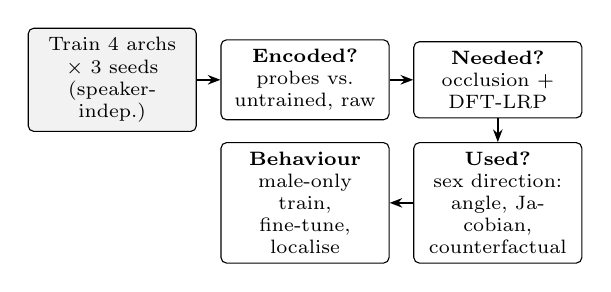
\begin{tikzpicture}[
  node distance=3mm and 3mm,
  box/.style={draw, rounded corners=2pt, align=center, font=\scriptsize,
              minimum height=8mm, text width=19mm},
  arr/.style={-{Stealth[length=1.6mm]}, thick}]
\node[box, fill=gray!10] (train) {Train 4 archs\\$\times$ 3 seeds\\(speaker-indep.)};
\node[box, right=of train] (enc) {\textbf{Encoded?}\\probes vs.\\untrained, raw};
\node[box, right=of enc] (inp) {\textbf{Needed?}\\occlusion +\\DFT-LRP};
\node[box, below=of inp] (rep) {\textbf{Used?}\\sex direction:\\angle, Jacobian,\\counterfactual};
\node[box, left=of rep] (beh) {\textbf{Behaviour}\\male-only train,\\fine-tune,\\localise};
\draw[arr] (train) -- (enc);
\draw[arr] (enc) -- (inp);
\draw[arr] (inp) -- (rep);
\draw[arr] (rep) -- (beh);
\end{tikzpicture}
\caption{Study design. Every test has a control: untrained networks and raw
input for probing, random/least-relevant removal for attribution, an
exhaustive split null and random directions for the sex direction, and a
size-matched male-only control for behaviour.}
\label{fig:pipeline}
\end{figure}

\begin{figure*}[!t]
\centering
\begin{minipage}[b]{0.28\textwidth}\centering\paperfig[\linewidth]{\FigSexAccent}\\[1pt]{\footnotesize (a)}\end{minipage}\hspace{0.06\textwidth}
\begin{minipage}[b]{0.43\textwidth}\centering\paperfig[\linewidth]{\FigFzero}\\[1pt]{\footnotesize (b)}\end{minipage}
\caption{AudioMNIST speakers. (a) Sex $\times$ accent counts: German accents
dominate and most cells hold one speaker. (b) Median F0 per utterance by sex.}
\label{fig:data}
\end{figure*}

\subsection{Data}
AudioMNIST \cite{becker2024audiomnist} contains 30{,}000 recordings of the
digits 0--9 spoken by 60 speakers (48 male, 12 female), 50 repetitions each;
41 of 60 speakers have a German accent (Fig.~\ref{fig:data}). Pitch alone
nearly separates the sexes: median F0 per utterance clusters around
100--150\,Hz for male and 180--260\,Hz for female speakers. Each 48\,kHz
recording is resampled to 8\,kHz (librosa, soxr), centre zero-padded to 8{,}192
samples (1.024\,s; no recording is longer) and peak-normalised. No data
augmentation is used.

We use a \emph{speaker-independent} (SI) split, in which test speakers are
never heard during training. It is built by stratified group 5-fold
partitioning (speakers as groups, stratified by sex, seed 42): one fold is
the test set (12 speakers: 3 female, 9 male), one the validation set (12: 2
female, 10 male) and three the training set (36: 7 female, 29 male; 18{,}000
recordings). The validation set is used for early stopping and checkpoint
selection. The same split serves every architecture and seed. A
\emph{speaker-dependent} (SD) split, a random 60/20/20 split of recordings
stratified by digit in which every speaker appears on both sides, serves only
as a diagnostic for voice memorisation. An automated test enforces zero
speaker overlap in the SI split. Because recordings from one person are not
independent, group metrics are computed per speaker: the effective sample
size is 12 people, not thousands of recordings. All analyses use the three
SI test women, except fine-tuning (Section~\ref{sec:ft}), which rotates
held-out women over four folds of three so that all 12 are evaluated.

\subsection{Implementation}

\begin{table}[t]
\caption{Training and analysis settings}
\label{tab:params}
\centering\footnotesize
\setlength{\tabcolsep}{3pt}
\begin{tabular}{@{}lp{5.3cm}@{}}
\toprule
Item & Setting \\
\midrule
Input & 8\,kHz, 8{,}192 samples, peak-normalised; no augmentation \\
SI split & Train/val/test 36/12/12 speakers (7/2/3 female), seed 42 \\
Training & Cross-entropy; Adam, lr $10^{-3}$; batch 128; $\le$8 epochs; patience 3 on val.\ accuracy \\
Probes & Standardised features; logistic regression, L2, $C=1$, L-BFGS, 2{,}000 iterations \\
Sex probe & Train 48 speakers (train+val), test 12 SI test speakers \\
Identity probe & 70/30 split of each speaker's recordings \\
Occlusion & 16 bands $\times$ 250\,Hz; DFT-bin zeroing; 6{,}000 recordings \\
DFT-LRP & zennit \texttt{EpsilonPlusFlat} (flat / $z^{+}$ / $\varepsilon=10^{-6}$); predicted class; 1{,}000 recordings \\
Faithfulness & 5\% steps of 4{,}097 DFT bins, zero replacement; AUC \\
Sex direction & Logistic probe on standardised penultimate activations; 219-split null; Procrustes \\
Sensitivity & 1{,}000 random unit directions \\
Counterfactual & $\delta\in[-3,3]$, 11 values; correctly classified recordings \\
Acoustics & pYIN F0 65--300\,Hz; Burg formants, 5, 3.8\,kHz \\
Fine-tuning & All layers; Adam, lr $10^{-4}$; batch 128; 2 epochs \\
Bootstrap & 1{,}000 resamples over speakers \\
\bottomrule
\end{tabular}
\end{table}

All models are implemented in PyTorch \cite{paszke2019pytorch}.

\emph{Architectures.} (1) \texttt{cnn1d} reads the raw waveform with five
convolutional blocks (32, 64, 128, 128 and 256 channels; kernels 9, 5, 3, 3,
3), each followed by batch normalisation, ReLU and max-pooling by 4. Global
average pooling gives a 256-dimensional penultimate vector, followed by
three fully connected layers (128, 64, 10 units; ReLU, dropout 0.3); 226k
parameters. (2) \texttt{resnet1d} uses the same channels and kernels but adds
a residual shortcut (a $1\times1$ convolution where the width changes) to
each block before the ReLU \cite{he2016resnet}; 270k parameters. (3)
\texttt{crnn\_gru} uses the first three \texttt{cnn1d} blocks followed by a
two-layer GRU \cite{cho2014gru} (hidden size 128, dropout 0.3) whose final
hidden state is the 128-dimensional penultimate vector; 235k parameters. (4)
\texttt{spec\_cnn2d} applies four 2-D convolutional blocks (24, 48, 96, 128
channels, $3\times3$ kernels, batch normalisation, ReLU, $2\times2$
max-pooling), global average pooling to 128 dimensions and the same
three-layer head; 189k parameters. Its input is a 64-band log-mel spectrogram
(FFT size 256, Hann window, hop 128, 0--4\,kHz, power in dB relative to each
recording's maximum and floored at $-80$\,dB), giving $64\times65$
time--frequency bins.

\emph{Training.} All four share one protocol (Table~\ref{tab:params}):
cross-entropy loss, Adam with learning rate $10^{-3}$ and no weight decay,
batch size 128, at most 8 epochs, and early stopping with patience 3 on
validation accuracy, keeping the best checkpoint. Each is trained from seeds
42, 43 and 44 with deterministic algorithms; runs stopped after 5--8 epochs.
Training and most analyses ran on a laptop CPU; band occlusion, DFT-LRP, the
within-digit geometry and the seed-43/44 probing ran on a GPU server.

\emph{Probing (RQ1).} We freeze each network and record the output of each
block (after ReLU and pooling), averaged over time (and frequency for
\texttt{spec\_cnn2d}), together with the penultimate vector. Features are
standardised with statistics from the probe-training data and passed to an
L2-regularised logistic regression (scikit-learn, $C=1$, L-BFGS, at most
2{,}000 iterations). The sex probe is trained on the 48 SI training and
validation speakers and tested on the 12 held-out test speakers (majority
chance 0.75), so success reflects encoding rather than memorising
individuals. A 60-way identity classifier cannot name speakers it never saw,
so the identity probe measures \emph{re-identification}: it is trained on
70\% of each speaker's recordings and tested on the other 30\% (chance 1/60).
The same probes are fit on (a) a copy of the architecture with PyTorch's
default random initialisation, frozen, and (b) for \texttt{cnn1d}, a raw-input
baseline: the time-averaged 64-band log-mel spectrum. The \emph{margin} is
trained minus untrained probe accuracy: a margin near zero means training
added nothing. Linear CKA \cite{kornblith2019cka} compares penultimate
representations across architectures on 4{,}000 random recordings.

\emph{Input level (RQ2).} Band occlusion sets to zero all bins of one of 16
bands of 250\,Hz (0--4\,kHz) in the 8{,}192-point real DFT of the waveform,
inverts the transform (for \texttt{spec\_cnn2d} the spectrogram is
recomputed from the occluded waveform) and records the drop in digit accuracy
over the 6{,}000 SI test recordings (\emph{necessity}). DFT-LRP
\cite{vielhaben2024virtual} attributes the predicted class to frequency bins:
LRP relevance of the waveform is mapped onto its real DFT (rectangular window,
4{,}097 bins) by a virtual inspection layer. We use the zennit
\texttt{EpsilonPlusFlat} composite with batch normalisation merged into the
preceding convolution: the flat rule for the first convolution, the
$z^{+}$ rule for the remaining convolutions and the $\varepsilon$-rule
($\varepsilon=10^{-6}$) for fully connected layers, with relevance passed
through ReLU and pooling. Absolute bin relevance is averaged over 1{,}000
random test recordings and summed into the 16 bands. Faithfulness is checked
by zeroing bins in 5\% steps in most-relevant-first (MoRF),
least-relevant-first (LeRF) and random order and integrating the
predicted-class probability (AUC) \cite{samek2017evaluating}; the attribution
passes if MoRF falls fastest. DFT-LRP is applied to the two waveform CNNs,
whose layers these rules cover.

\emph{Representation level (RQ3).} We rank penultimate units by female--male
selectivity (Cohen's $d$ on the SI test recordings) and compare the top-20
units (Jaccard overlap against its chance value) and full rankings (Spearman
$\rho$) across seeds; PCA gives the variance share of the top ten components.
We then estimate a sex direction $\hat{u}$: a logistic probe (as above) is fit
on the per-unit standardised penultimate activations of the 12 SI test
speakers, and its weight vector is mapped back to the original coordinates
and normalised. To test that $\hat{u}$ is specific to sex, rather than to any
3-vs-9 grouping of these 12 speakers, we refit it for each of the
$\binom{12}{3}-1=219$ alternative 3-vs-9 groupings and compare cross-seed
reproducibility (cosine after orthogonal Procrustes alignment of the seeds'
penultimate spaces). Use is then tested in three ways. (a) \emph{Geometry.}
At the penultimate layer we measure the angle between the mean of ten
per-digit sex-probe directions (trained on the 48 training and validation
speakers) and the subspace spanned by the ten digit class means. At every
layer we measure the angle between that layer's sex-probe direction and the
dominant direction of the per-recording gradients of the correct-digit logit.
(b) \emph{Sensitivity.} The mean Jacobian of the trained head's logits with
respect to the penultimate vector is projected on $\hat{u}$ and expressed, per
digit, as a percentile of 1{,}000 random unit directions. (c)
\emph{Counterfactual.} We add $\delta\cdot\Delta\,\hat{u}$ to the penultimate
vector of every correctly classified test recording, where $\Delta$ is the
female--male gap in mean projection and $\delta$ takes 11 values in
$[-3,3]$, and record the correct-digit logit and accuracy. To characterise
$\hat{u}$ acoustically, we extract F0 with pYIN (65--300\,Hz) and F1--F3 with
Praat's Burg method (five formants, ceiling 3.8\,kHz) from the 8\,kHz input,
and correlate each recording's projection onto $\hat{u}$ with them
(Spearman). The decisive test is within the nine male speakers, which does
not depend on the three women.

\emph{Behaviour (RQ4).} For \texttt{cnn1d} and \texttt{spec\_cnn2d} we train
a male-only model (38 male training and 10 male validation speakers, same
protocol, three seeds) and test it on women. The SI baseline was trained on
seven of the 12 women and validated on two, so the comparison is restricted to
the three SI test women, whom neither model heard, with speaker-level
bootstrap intervals; it is repeated leaving out each of them in turn. The
control trains new models on 38 men, matching the male-only model's size, and
compares them with the SI baseline on the nine SI test men. Finally, we
fine-tune the male-only model on women. The 12 women form four folds; each
fold fine-tunes on nine and evaluates on the other three. Fine-tuning updates
all weights with Adam at learning rate $10^{-4}$ and batch size 128 for a
fixed two epochs, without early stopping, so that conditions are directly
comparable; a pilot showed no further gain from a third epoch. In a control
condition the same fine-tuning is applied to men: the male-only model's ten
validation speakers (used only for checkpoint selection), split into
fine-tuning and evaluation sets of 7--8 and 2--3. We localise the change by
the relative $L_2$ change of each layer's activations on the evaluation
recordings, and, for \texttt{cnn1d}, by DFT-LRP band relevance before and
after fine-tuning.

\subsection{Evaluation plan}
Table~\ref{tab:rqmap} maps each research question to its evidence.
Uncertainty is reported as bootstrap intervals over speakers (1{,}000
resamples), ranges over
the three seeds, the exhaustive 219-split null and the 1{,}000-direction
null. Hypotheses for the confirmatory experiments were written down before
running them; one of them (that the sex direction is a pitch axis) was
falsified, and we report it as such.

\begin{table}[t]
\caption{Research questions, methods and evidence}
\label{tab:rqmap}
\centering\footnotesize
\begin{tabular}{@{}lp{2.6cm}p{3.6cm}@{}}
\toprule
RQ & Method & Metric / control \\
\midrule
RQ1 & Layer-wise linear probes & Probe acc.; margin vs.\ untrained and raw input \\
RQ2 & Band occlusion, DFT-LRP & Accuracy drop per band; relevance share; MoRF/LeRF AUC \\
RQ3 & Units, sex direction & Top-20 overlap; 219-split null; angle; Jacobian percentile; counterfactual accuracy \\
RQ4 & Male-only training, fine-tuning & Accuracy drop vs.\ same-size control; layer change; band change \\
\bottomrule
\end{tabular}
\end{table}

\subsection{Risks and limitations}
\emph{(1) Three women.} Each test fold holds three female speakers, so every
sex-related result is a within-sample claim about those speakers and not a
population estimate. \emph{(2) No clean control for adaptation.} AudioMNIST
has no unseen males comparable to the unseen women (male controls are at
ceiling), so we cannot separate female-specific adaptation from generic
new-speaker adaptation. \emph{(3) Linear read-outs.} Non-linear use of sex is
not excluded. \emph{(4) Partial architecture coverage.} The sex direction is
validated in two of four architectures, and the GRU's penultimate sex probe
is at chance. \emph{(5) Accent and age} cannot be assessed on this dataset.

% =====================================================================
\section{Results}\label{sec:results}

\begin{figure}[!t]
\centering
\begin{minipage}[b]{0.48\linewidth}\centering\paperfig[\linewidth]{\FigLeakage}\\[1pt]{\footnotesize (a)}\end{minipage}\hfill
\begin{minipage}[b]{0.48\linewidth}\centering\paperfig[\linewidth]{\FigAccBySex}\\[1pt]{\footnotesize (b)}\end{minipage}
\caption{(a) Digit accuracy on unseen (SI) vs.\ familiar (SD) speakers.
(b) Speaker-level accuracy by sex with 95\% intervals ($n=3$ female, 9 male).}
\label{fig:baseline}
\end{figure}

\begin{figure*}[!t]
\centering
\begin{minipage}[b]{0.41\textwidth}\centering\paperfig[\linewidth]{\FigProbeSex}\\[1pt]{\footnotesize (a)}\end{minipage}\hspace{0.06\textwidth}
\begin{minipage}[b]{0.41\textwidth}\centering\paperfig[\linewidth]{\FigProbeId}\\[1pt]{\footnotesize (b)}\end{minipage}
\caption{Layer-wise linear probe accuracy for (a) sex (held-out speakers)
and (b) speaker re-identification (held-out recordings of known speakers) in
the 1-D CNN: trained, untrained control, raw-input baseline and chance.}
\label{fig:probes}
\end{figure*}

\subsection{The model is accurate and looks fair}
The 1-D CNN reaches 95.5\% digit accuracy on unseen speakers and 98.7\% on
familiar ones (Fig.~\ref{fig:baseline}a). The 3.3-point gap is voice
memorisation that does not transfer, and is a lower bound because training
stopped early. The confusion matrix has a strong diagonal; digit 9 is the
hardest and is confused with 7, 0 and 1. Speaker-level accuracy is 0.914
[0.770, 0.998] for the three female and 0.968 [0.940, 0.990] for the nine
male test speakers (Fig.~\ref{fig:baseline}b). The intervals overlap, so no
sex difference can be claimed: a standard audit would pass this model.

\subsection{Speaker sex is encoded, but inherited from the audio}
Linear probes read sex from the trained 1-D CNN at up to 0.99 (conv3), and
re-identify known speakers from unseen recordings at up to 0.92
(Fig.~\ref{fig:probes}). But the untrained
network and the raw input read sex about equally well ($\approx$0.97, chance
0.75): the digit task did not create this information. Speaker identity
behaves differently. It rises to a peak in the middle of the network and then
falls as the final layers specialise for the digit, ending well below the raw
input (0.94) but not at chance.

At the penultimate layer of all four architectures, training adds no sex
decodability beyond random initialisation (Table~\ref{tab:margins}). Across
three seeds the sex margin is negative or near zero in every architecture
($-0.06$ to $-0.01$), whereas the identity margin is positive (about $+0.08$
to $+0.13$ for the convolutional models and $+0.38$ for the GRU;
Table~\ref{tab:margins}, with seed ranges in Fig.~\ref{fig:app}a). Sex is inherited; identity is partly induced.

The architectures are not simply copies of one another: linear CKA between
penultimate representations is 0.93 for the two waveform CNNs but 0.60--0.69
for every other pair. The same inheritance pattern across genuinely different
representations suggests it is a property of the signal, not of one design.

\begin{table}[t]
\caption{Penultimate linear-probe accuracy (seed 42) and trained-minus-untrained margins (mean of seeds 42/43/44)}
\label{tab:margins}
\centering\footnotesize
\setlength{\tabcolsep}{4pt}
\begin{tabular}{@{}lccccc@{}}
\toprule
 & \multicolumn{3}{c}{Sex, seed 42} & \multicolumn{2}{c}{Margin, 3 seeds} \\
\cmidrule(lr){2-4}\cmidrule(l){5-6}
Architecture & Trained & Untr. & Margin & Sex & Identity \\
\midrule
1-D CNN         & 0.94 & 0.97 & $-0.04$ & $-0.06$ & $+0.09$ \\
Residual CNN    & 0.96 & 0.98 & $-0.02$ & $-0.03$ & $+0.08$ \\
GRU-CRNN        & 0.74 & 0.75 & $-0.01$ & $-0.01$ & $+0.38$ \\
Spectrogram CNN & 0.92 & 0.95 & $-0.02$ & $-0.03$ & $+0.13$ \\
\bottomrule
\end{tabular}\\[2pt]
{\scriptsize Chance for sex = 0.75. Seed ranges in Fig.~\ref{fig:app}a.}
\end{table}

\begin{figure*}[!t]
\centering
\begin{minipage}[b]{0.40\textwidth}\centering\paperfig[\linewidth]{\FigNecessity}\\[1pt]{\footnotesize (a)}\end{minipage}\hfill
\begin{minipage}[b]{0.58\textwidth}\centering\paperfig[\linewidth]{\FigDftLrp}\\[1pt]{\footnotesize (b)}\end{minipage}
\caption{(a) Necessity: digit-accuracy drop when each 250\,Hz band is silenced,
all four architectures (seed 42), pitch and formant regions shaded.
(b) Necessity (occlusion drop) and attribution ($|$DFT-LRP$|$) per band,
each normalised, for \texttt{cnn1d} and \texttt{resnet1d}.}
\label{fig:freq}
\end{figure*}

\subsection{Digit recognition needs formants, not pitch}
Silencing one 250\,Hz band at a time shows that digit accuracy depends
almost entirely on energy below about 1\,kHz, with the largest drops in the
250--750\,Hz formant region in all four architectures
(Fig.~\ref{fig:freq}a). Above 1.5\,kHz, removing a band costs the 1-D CNN
and the GRU less than one point, the residual CNN at most 1.5 points and the
spectrogram CNN up to 3.4 points, against peaks of 4.6--25 points below
750\,Hz. The pitch band (0--250\,Hz), the strongest sex cue, is comparatively
dispensable.

DFT-LRP, computed for the two waveform CNNs, agrees: 88--90\% of the
absolute relevance lies below 750\,Hz, and the attribution and necessity
profiles correlate at $r=0.62$ (\texttt{cnn1d}) and $0.67$
(\texttt{resnet1d}; Fig.~\ref{fig:freq}b). The attribution is faithful: for
\texttt{cnn1d}, removing the most relevant bins first destroys the prediction
far faster (AUC 0.15) than random (0.41) or least-relevant-first removal
(0.54; Fig.~\ref{fig:app}b), and \texttt{resnet1d} gives almost the same
values (0.16, 0.39, 0.55). The two methods differ in one place:
DFT-LRP assigns the largest single share to the 0--250\,Hz band, while
occlusion shows that removing it costs less than removing 250--750\,Hz. The
pitch band is therefore weighted but redundant: the model reads it, but can
do without it. Splitting the
necessity profiles by speaker sex shows similar shapes (profile correlation
$r=0.41$--$0.93$), diverging most around 625\,Hz; with three women, we treat
this difference as low-to-medium confidence.

\subsection{There is no sex neuron, but there is a sex direction}
Voice information survives within each digit: inside every single digit, sex
can be decoded at 0.94--0.95 on average in the three convolutional models
(the GRU reaches 0.80, near the 0.75 majority rate, and is excluded from the
following direction analyses). No individual unit carries it reliably. The
most female-selective penultimate units change completely when the model is
retrained: top-20 overlap across seeds is at chance and the full ranking
correlates at $\rho\approx0$. The reason is structural. PCA puts 94--98\% of
penultimate variance in about ten directions, so units are interchangeable
coordinates in a near-rank-10 space rather than fixed detectors.

We therefore move from units to a direction. A raw mean-difference
direction turned out to be confounded: in a rank-10 space it matches almost
any contrast between groups of these 12 speakers. The probe direction fit on
standardised activations resolves this. Its cross-seed reproducibility exceeds all 219
alternative 3-vs-9 re-splits in \texttt{cnn1d} and \texttt{spec\_cnn2d}, but
falls inside the null for \texttt{resnet1d} and the GRU (Fig.~\ref{fig:app}c).
We continue with the two validated models. This removes the metric
confound but not the sample one: the direction is sex-specific across these
12 speakers, and its generality beyond three women cannot be tested.

\subsection{The sex direction is not a pitch axis}
We pre-registered that the direction would track F0. Across sexes, the
projection correlates with F0 at $\rho=0.66$ and $0.64$, but only because the
sexes form two separate clusters (Fig.~\ref{fig:app}d). Within the nine
male speakers the correlation is $\rho=0.19$ (\texttt{cnn1d}) and $0.13$
(\texttt{spec\_cnn2d}), explaining 2--4\% of variance, and within women it is
0.06--0.08. The prediction is falsified: the direction separates the sexes
categorically, using more than pitch or formants. We can say what it is not,
but not yet which acoustic property it is.

\subsection{The digit decision does not use the sex direction}
\begin{figure*}[!t]
\centering
\begin{minipage}[b]{0.49\textwidth}\centering\paperfig[\linewidth]{\FigJacobian}\\[1pt]{\footnotesize (a)}\end{minipage}\hfill
\begin{minipage}[b]{0.49\textwidth}\centering\paperfig[\linewidth]{\FigCounterfactual}\\[1pt]{\footnotesize (b)}\end{minipage}
\caption{(a) Readout sensitivity to the sex direction per digit, as a
percentile of 1{,}000 random directions (seed 42). (b) Correct-digit logit
and accuracy when representations are shifted along the sex direction by
$\delta$ times the male--female gap.}
\label{fig:use}
\end{figure*}

Three measurements agree. \emph{Geometry:} at the penultimate layer the mean
per-digit sex direction lies 82.5$^\circ$ (1-D CNN), 83.1$^\circ$ (residual
CNN) and 83.5$^\circ$ (spectrogram CNN) from the subspace spanned by the digit
class means, a spread of about one degree. At every layer of both validated
models, across all three seeds, the layer's sex-probe direction lies
79--90$^\circ$ from the dominant direction of the digit-logit gradients.
\emph{Sensitivity:} for seed 42, the readout's Jacobian along $\hat{u}$ sits
at or below the 35th percentile of 1{,}000 random directions for every digit
in both validated models (Fig.~\ref{fig:use}a). Across all 60 tests (3 seeds
$\times$ 2 architectures $\times$ 10 digits) it is below the median in 58,
reaches at most the 53rd percentile, and never exceeds the 95th, including
for the confusable digits 0, 1, 7 and 9. \emph{Counterfactual:} moving the representations of correctly
classified recordings along the direction by up to three times the full
male--female gap barely changes the correct-digit logit and changes accuracy
by less than 0.002
(Fig.~\ref{fig:use}b). The model encodes sex, but its decision stays out of
the way of the direction that carries it.

\subsection{Yet a model that never heard women reads them worse}\label{sec:behav}
Behaviour tells a different story. Relative to the SI baseline, a model
trained only on male speakers loses 7.9 (1-D CNN) and 5.0 (spectrogram CNN)
points on the three women neither model heard. A control trained on the same
number of men loses only 2.9 and 2.1 points on the nine held-out men
(Fig.~\ref{fig:maleonly}), and the female gap survives leaving out any one of
the three women. Restricting the comparison to these three women corrects a
confound: the SI baseline had trained or validated on the other nine. The
direction of the gap is stable across seeds; its size rests on three women.
Sex therefore matters somewhere, just not along the direction we measured.

\begin{figure}[!t]
\centering
\paperfig[0.62\linewidth]{\FigMaleOnly}
\caption{Accuracy gap relative to the speaker-independent baseline, for
\texttt{cnn1d} and \texttt{spec\_cnn2d}. Purple: trained without women,
tested on the three SI test women. Green: trained on the same number (38)
of men, tested on the nine SI test men.}
\label{fig:maleonly}
\end{figure}

\subsection{The gap is repaired by late-layer recalibration}\label{sec:ft}
\begin{figure*}[!t]
\centering
\begin{minipage}[b]{0.55\textwidth}\centering\paperfig[\linewidth]{\FigFtRecovery}\\[1pt]{\footnotesize (a)}\end{minipage}\hfill
\begin{minipage}[b]{0.43\textwidth}\centering\paperfig[\linewidth]{\FigFtBands}\\[1pt]{\footnotesize (b)}\end{minipage}
\caption{(a) Change in digit accuracy from fine-tuning (after minus before),
per fold, for held-out women (red) and the male control (blue); error bars show
the min--max over seeds 42/43/44. (b) Relative change in DFT-LRP relevance per
frequency band after fine-tuning, female vs.\ male control (\texttt{cnn1d};
min--max over seeds and folds).}
\label{fig:ft}
\end{figure*}

Fine-tuning the male-only model on women recovers the gap: on average, female
accuracy rises from 0.87 to 0.96 (+9 points, 1-D CNN) and from 0.86 to 0.96
(+11, spectrogram CNN). Repeating the 1-D CNN fine-tuning on the GPU server
reproduced post-fine-tuning accuracy within 0.7 points. The gain is positive
in all four folds of both models, although small in one \texttt{cnn1d} fold,
while the same fine-tuning applied to men changes accuracy by close to zero
(Fig.~\ref{fig:ft}a). Comparing activations on female speech before and
after fine-tuning shows that the change concentrates in the late,
decision-adjacent layers, and barely touches the acoustic front-end. DFT-LRP
confirms this independently for \texttt{cnn1d}: on female speech, reliance
falls by a similar proportion in every 250\,Hz band, between about $-15\%$
and $-27\%$, with no band singled out, while the male control stays near
zero (Fig.~\ref{fig:ft}b). Fine-tuning does not make the model listen
to different frequencies; it recalibrates how already-extracted evidence is
combined into a digit.

% =====================================================================
\section{Conclusion}\label{sec:conclusion}

We asked whether spoken-digit classifiers that encode speaker sex also use it
to classify digits, and tested \emph{encoded} and \emph{used} as separate
claims. Sex is encoded in every architecture, but it is inherited from the
audio rather than created by training. At the input, digit recognition relies
on the formant region and can do without the pitch band that carries the
strongest sex cue. In the representation, sex directions stay close to
orthogonal to the digit decision at every layer, the readout is no more
sensitive to the validated sex direction than to random directions, and
accuracy is unchanged when representations are shifted along it. In behaviour, a model that never heard women still reads them
worse, and the repair happens in the late layers that combine evidence, not
in the layers that extract it. The representational tests address one
estimated direction, while the behavioural test catches any route, so the two
results do not contradict each other: the model knows who is speaking, does
not read the digit through that knowledge, and adapts to unfamiliar voices by
recalibrating its decision layers.

Three lessons carry beyond this dataset. First, output parity, probing and
attribution answer different questions, and a fairness claim needs the
evidence that matches it. Second, untrained-network controls are needed to
read probing results: high decodability of a protected attribute says little
about what training did. Third, because speaker information is separable in
the representation but not in the input, concept-direction methods offer more
leverage for explanation than further input-level attribution. All
sex-related estimates rest on three held-out women, and whether the recovered
machinery is specific to women or generic new-speaker adaptation cannot be
decided on AudioMNIST.

% =====================================================================
\section{Future Work}\label{sec:future}

Four directions follow from these results and their limits.

\emph{Breaking the three-women ceiling.} Every sex-related estimate here rests
on three held-out female speakers. Repeating the protocol on a speech corpus
with many speakers of each sex and recorded speaker metadata would turn the
within-sample claims into population estimates. It would also supply the
missing control, unseen male speakers, which is needed to decide whether the
late-layer recalibration of Section~\ref{sec:ft} is specific to women or is
generic adaptation to new voices.

\emph{Naming the sex direction.} The validated direction is categorical and
is not a pitch axis, but its acoustic content is unknown. Concept-level
attribution such as Concept Relevance Propagation \cite{achtibat2023crp},
together with formant, spectral-tilt and voice-quality measures, could
identify what the direction is made of, and explain why it is validated in
\texttt{cnn1d} and \texttt{spec\_cnn2d} but not in \texttt{resnet1d} or the
GRU.

\emph{From geometry to causal tests.} Our evidence of non-use is linear and
bounded to one estimated direction. Removing the sex subspace by iterative
nullspace projection \cite{ravfogel2020inlp} or amnesic probing
\cite{elazar2021amnesic}, and repeating the tests with non-linear probes,
would check whether any other route carries sex into the digit decision, and
could locate the route behind the behavioural gap.

\emph{Clinical time series.} The protocol does not depend on audio. The AAI
Lab at Technische Hochschule Mittelhessen plans to extend this work to ECG
classifiers, asking whether models trained on a clinical label encode patient
sex or age, and whether their decisions use them. There, the gap between
output parity and internal use has direct consequences for patients.

% =====================================================================
\section*{Code and Data Availability}

The code, configurations, saved results and figure scripts for this paper
are available at \repourl. The AudioMNIST dataset \cite{becker2024audiomnist}
is available at \url{https://github.com/soerenab/AudioMNIST}.

% =====================================================================
\FloatBarrier % main-text figures appear before the appendix

\bibliographystyle{IEEEtran}
\bibliography{refs}

% =====================================================================
\appendices
\renewcommand{\thefigure}{A\arabic{figure}}
\setcounter{figure}{0}

\begin{figure*}[!p]
\centering
{\normalsize\scshape Appendix: Supporting Figures\par}\vspace{8pt}
\paperfig[0.88\textwidth]{\FigSeedMargins}\\
{\footnotesize (a)}\\[6pt]
\begin{tabular}{@{}c@{\hspace{0.04\textwidth}}c@{}}
\paperfigh[2.25in]{\FigFaithful} & \paperfigh[2.25in]{\FigSplitNull} \\
{\footnotesize (b)} & {\footnotesize (c)} \\
\end{tabular}\\[6pt]
\paperfig[0.88\textwidth]{\FigFzeroProj}\\
{\footnotesize (d)}
\caption{Supporting results cited in Section~\ref{sec:results}. (a) Trained-minus-untrained probe margins for sex
(left) and speaker identity (right), mean and range over seeds 42/43/44.
(b) DFT-LRP faithfulness for \texttt{cnn1d}: mean predicted-class probability
as frequency bins are removed in MoRF, random and LeRF order. (c) Cross-seed
reproducibility of the sex direction $\hat{u}$ (red) against all 219
alternative 3-vs-9 splits of the same 12 speakers (grey); dashed: the
confounded raw mean-difference direction. (d) Projection of each clip onto
the sex direction $\hat{u}$ vs.\ median F0 for \texttt{cnn1d} and
\texttt{spec\_cnn2d}; blue: male (9 speakers), red: female (3 speakers).}
\label{fig:app}
\end{figure*}

\end{document}